\documentclass{article}

\usepackage{geometry}
\usepackage{float}
\usepackage{caption}
\geometry{a4paper}
\usepackage{amsmath}
\usepackage{graphicx}
\usepackage[obeyspaces]{url}
\usepackage{listings}
\usepackage[space]{grffile}
\usepackage[toc,page]{appendix}

\title{Interim Report\\
Prediction of Crime Patterns in Chicago\vfill{}}

\author{Submitted By:\\Ravisutha Sakrepatna Srinivasamurthy\\
						Saroj Kumar Dash}

\begin{document}
	\begin{titlepage}
		\maketitle
		\pagenumbering{gobble}
		\end{titlepage}
	
\newpage

\tableofcontents

\newpage	

\pagenumbering{arabic}

\section{Introduction}
In this project we are analyzing the Chicago Crime Data \cite{data}. Following section explains our objective, intended method for achieving the objective and progress until today.

\section{Objective}
Our objective is to predict crime pattern in Chicago (lets say for next year) by using data from previous years with the help of network analysis techniques.

\section{Approach}
We are currently contemplating on different methods by which we can achieve our objective. But before applying any method, we are facing some design challenges; namely how to construct a network and what forms a node etc. We have various datasets such as education dataset, income dataset, rider dataset, etc. Our first challenge is to come up with a network using these datasets.

\subsection{Building network}
\paragraph{}
We are currently considering crime data for the year 2015. We will use data from this year to test out all intended methods and to analyze them . And then we will extend it to other years. In 2015, there were 263,477 reported crimes. Each crime will be treated as a node. There are total of 401 crime types  according to Chicago Police website\cite{police}. And crime can happen either in morning, or afternoon or night or in the early morning. Based on these, we have 401 types crime that can happen in 4 different times of a day. We will consider each of these combination as a node. Hence we will end up with 1604 more nodes. Again, we will divide the crime based on months. This will add 12 * 401 = 4804 more nodes to our network. Each crime is associated with an area. Chicago can be divided based on many attributes such as ward number, precinct, district, etc. Our choice depends on the other datasets as explained below.
\paragraph{}
Along with crime dataset, we will be using education, rider, income and police beats datasets. But some of these datasets are based on wards and some are based on precincts etc. We have to somehow unify these datasets and then we have to incorporate in our network. We are currently working on this.
\subsection{Methods to predict next crime pattern}
We are currently contemplating three methods to achieve our objective. 
\begin{itemize}
\item First method is to build network for different years (let's say 2001 and 2002). Then compare these to networks and analyze the changes. We are hoping to use Laplace inverse matrix\cite{rwalk} to find the dissimilarity in the network and analyze the network based on this matrix. And based on these analysis predict the crime trends for future years.
\item Second method is to predict the spread of crime from one area to another area. This is similar to network analysis of how an epidemic disease spreads in a network\cite{spread}. This analysis will help in predicting the spread of crime to other areas.
\item And finally, in a given year, we want to see what influences the observed crime pattern. For this we intend to use role discovery algorithm that was presented by one of our peer in the class. This may or may not work but we are curious about what this algorithm may come up with.
\end{itemize}

\subsection{Progress}
We are currently cleaning the dataset and trying to build the network. We got a network just by using the crime dataset(Figure \ref{fig:fig1}). Nodes for this network are community and crime types.
\begin{figure}
	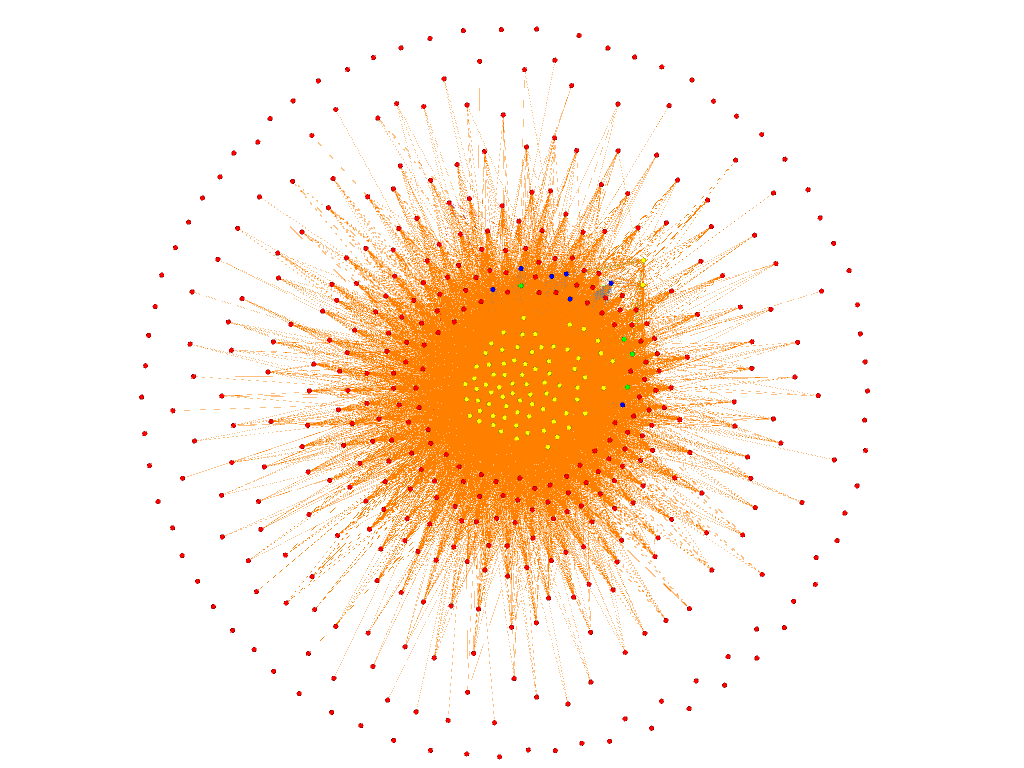
\includegraphics[scale=0.4, trim={0 0.5cm 0 6cm}]{network_vis.png}
	\caption{Visualization of crime network. Red nodes are crime types, yellow nodes are the community, green nodes are time of the day and blue nodes represents weekday. This is a preliminary network. Our network will change after we incorporate changes as described in the above sections.}
	\label{fig:fig1}
\end{figure}

We are currently trying to unify all other datasets so that it can incorporated in the network as explained in the above subsection.

\subsection{Timeline}
This is our expected timeline leading to the completion of the project.
\begin{itemize}
\item Cleaning the data and building the network should be complete by 11/12/2017
\item Apply the three methods and analyze the network by 19/12/2017
\item Predict the future crime trends by 11/22/2017
\item Get feedback from Dr. Safro and make necessary changes. 11/24/2017
\item Prepare the report and submit by 11/27/2017
\end{itemize}

\begin{appendices}
 \chapter{Appendix A}
 \label{appendix:a}
 :Make network python code: 
 \lstinputlisting[language=Python]{"/home/ravi/Network_Science/Project/Code/make_network.py"}
\end{appendices}

\begin{thebibliography}{9}

\bibitem{role} Ahmed, N.~K., Rossi, R.~A., Willke, T.~L., \& Zhou, R.\ 2016, arXiv:1610.00844 
\bibitem{rwalk} F. Fouss, A. Pirotte, J. m. Renders and M. Saerens, "Random-Walk Computation of Similarities between Nodes of a Graph with Application to Collaborative Recommendation," in IEEE Transactions on Knowledge and Data Engineering, vol. 19, no. 3, pp. 355-369, March 2007.
\bibitem{spread}https://www.theatlantic.com/magazine/archive/2013/10/violence-is-contagious/309459/
\bibitem{data}https://data.cityofchicago.org/Public-Safety/Crimes-2001-to-present/ijzp-q8t2
\bibitem{police}https://data.cityofchicago.org/Public-Safety/Chicago-Police-Department-Illinois-Uniform-Crime-R/c7ck-438e
\end{thebibliography}
\end{document}